\documentclass{article}
%packages
\usepackage{graphicx}
\usepackage{hyperref}
\usepackage[utf8]{inputenc}
\usepackage[T1]{fontenc}
\usepackage[a4paper]{geometry}
\usepackage{minted}

\title{Layer 802.15.4 for LoRa Fabian}
\date{July 21st 2015}

\begin{document}
\maketitle
\section{Architecture}
\subsection{Global functioning}
This documentation explains the implementation of the layer 802.15.4 between the radio layer and the contiki application. The main file is \emph{layer802154\_radio\_lora.h} [Figure~: \ref{fig:architecture}].\\
\begin{figure}[h]
	\begin{center}
		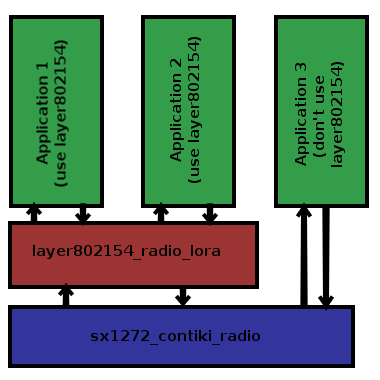
\includegraphics[scale=0.5]{img/archi}
		\caption{Layer 802.15.4}
		\label{fig:architecture}
	\end{center}
\end{figure}
This file provides the following functions:
\begin{minted}{c}
int layer802154_init(void);
\end{minted}
Init the layer.
\begin{minted}{c}
int layer802154_on(void);
\end{minted}
Turn on the layer.
\begin{minted}{c}
int layer802154_off(void);
\end{minted}
Stop the radio.
\begin{minted}{c}
int layer802154_channel_clear(void);
\end{minted}
Call the function channel\_clear() provided by the radio layer.
\begin{minted}{c}
frame802154_lora_t layer802154_read();
\end{minted}
Get and parse a 802.15.4 packet. A frame which contains the parsed packet is return.
\begin{minted}{c}
SIGNALISATION_ON //Signalisation flag for the header
SIGNALISATION_OFF
DST_SHORT_FLAG //Short mode address for destination address in the header
DST_LONG_FLAG

int layer802154_send(const void *payload, unsigned short payload_len,
 uint8_t* destAddr, int signalisation, int dstShortSrcLongFlag);
\end{minted}
Write the header and send the packet.\\
The function needs some parameters:
\begin{itemize}
  \item payload: The payload of the packet.
  \item payload\_len: The length of the payload.
  \item destAddr: The MAC address of the destination.
  \item signalisation: the signalisation flag of the header.
  \item dstShortSrcLongFlag: The mode for the length of the source and destination address.
\end{itemize}
\begin{minted}{c}
int layer802154_pending_packet(void);
\end{minted}
Return if a packet is present into the radio layer.
\subsection{802.15.4 packet specification}
The structure frame802154\_lora\_t provides:
\begin{minted}{c}
/**
 *  \brief: Structure that contains the Frame Control Field
 */
typedef struct {
  uint8_t _0_2_frame_type;       //3 bits
  uint8_t _3_security_enabled;   //1 bit
  uint8_t _4_frame_pending;      //1 bit
  uint8_t _5_ack_request;//1 bit
  uint8_t _6_pan_id_compression; //1 bit //HERE WE DO NOT RESPECT THE STANDARD! 
  We NEVER send PANID!
  //3 bits reserved
  uint8_t _10_11_dst_addr_mode;  //2 bits
  uint8_t _12_13_frame_ver;      //2 bits
  uint8_t _14_15_src_addr_mode;  //2 bits
} frame802154_lora_fcf_t;

/**
 * \brief: Structure that contains the 802.15.4 frame
 */
typedef struct {
  frame802154_lora_fcf_t fcf; //Frame control field
  uint8_t seq;//Sequence number
  uint8_t dest_addr[8];       //Destination address
  uint8_t src_addr[8];//Source address
  uint8_t *payload;   //Pointer to 802.15.4 frame payload
  uint8_t *packet;    //Pointer to all the packet
  int payload_len;    //Length of payload field
  int header_len;     //Length of header (-1 if an error occurs)
} frame802154_lora_t;
\end{minted}
Note~: dst\_addr\_mode must be different to src\_addr\_mode. The signalisation flag changes the last byte of the destination address. So, if the address is (0x00, 0x00), the message will contains (0x00, 0x80).\\
\begin{figure}[h]
	\begin{center}
		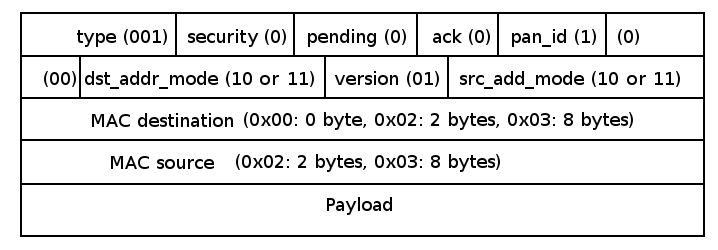
\includegraphics[scale=0.5]{img/trame}
		\caption{802.15.4 packet structure}
		\label{fig:trame802154}
	\end{center}
\end{figure}
\section{Using the layer}
The following code is present in the file \\
\emph{/platform/lorafabian/apps/frame\_manager/frame\_manager.c}
\subsection{Init the layer}
The 802.15.4 layer works like the radio layer. We can use the following functions:
\begin{minted}{c}
layer802154_init();
layer802154_on();
layer802154_off();
\end{minted}
\subsection{Read a packet}
\begin{minted}{c}
frame802154_lora_t frame = layer802154_read();
\end{minted}
The user have the access on a frame which contains the parsed packet. So he can access to the attributes previously described. He has also access to the functions\\\emph{int is\_broadcast\_addr(frame802154\_lora\_t *frame)} which check if the packet is a broadcast message \emph{int is\_my\_mac(frame802154\_lora\_t *frame)} which check if the destination MAC is the MAC of the contiki board (The MAC address is hardcoded in the file \emph{frame802154\_lora.c}).
\begin{minted}{c}
frame802154_lora_t frame = layer802154_read();
size = frame.payload_len;

if(frame.header_len == -1)
  printf("Error: buffer is too small for headers");
else {
  //For the arduino
  int packetSize = size + frame.header_len;
  //Verify the destination of a message
  bool br_msg = is_broadcast_addr(&frame);
  bool my_mac = is_my_mac(&frame);
  if(br_msg) {
    printf("Broadcast message");
    if(!is_signaling(&frame) || debug_on_arduino)
      set_arduino_read_buf(frame.packet, packetSize);
  }
  else if(my_mac) {
    printf("Message is for me");
    set_arduino_read_buf(frame.packet, packetSize);
  }
  else {
    printf("Message is not for me");
    if(debug_on_arduino)
      set_arduino_read_buf(frame.packet, packetSize);
  }
}
\end{minted}
\subsection{Send a packet}
This is how to send a COAP message:
\begin{minted}{c}
/**
 * \brief: Send the coap_payload_beacon to layer802154
 */
void
coap_beacon_send_response() {
  updateHOSTNAME();
  uint8_t tx_buffer[512];

  size_t coap_packet_size;
  static coap_packet_t coap_request[1];      //This way the packet can be treated as pointer as usual.

  unsigned short random_a = random_rand();
  char MAC[] = {0x00,0x00,0x00,0x00,0x00,0x00,0x00,0x00};
  getMac(MAC);
  unsigned short random_b = random_a ^ MAC[sizeof(MAC)-1];
  coap_init_message(coap_request, COAP_TYPE_NON, COAP_POST, (coap_get_mid()+random_b)%65535);
  int sizeMSG = strlen(coap_payload_beacon);
  coap_set_payload(coap_request, (uint8_t *)coap_payload_beacon, sizeMSG);

  coap_packet_size = coap_serialize_message(coap_request, (void *)(tx_buffer ));
  int tx_buffer_index = coap_packet_size;
  printf("We are sending the response to the coap beacon\n\r");

  //Note: We don't parse the beacon message yet, so the GATEWAY_ADDR
  //is defined in frame802154_lora.c
  layer802154_send(tx_buffer, tx_buffer_index, GATEWAY_ADDR, SIGNALISATION_ON, DST_SHORT_FLAG);

  //Note: We don't parse the beacon message yet, so we assume that
  //the node is registered after the first response
  is_associated = 1;
}
\end{minted}
\end{document}

